\documentclass[11pt,a4paper]{article}

\usepackage[headsep=1cm,headheight=3cm,left=3.5cm,right=3.5cm,top=2.5cm,bottom=2.5cm,a4paper]{geometry}

\linespread{1.3}
\setlength{\parindent}{0pt}
\setlength{\parskip}{1em}

\usepackage[spanish]{babel}
\usepackage[utf8]{inputenc}

%% Fuentes personalizadas para utilizar con XeTeX
\usepackage[sfdefault]{roboto}
\usepackage[scaled=0.9]{DejaVuSansMono}
\usepackage[T1]{fontenc}

\usepackage{enumitem}
\setlist[itemize]{leftmargin=*}
\setlist[enumerate]{leftmargin=*}

\usepackage{changepage}

\newcounter{ActCounter}
\newcommand{\act}[1]{\addtocounter{ActCounter}{1}\textbf{\sffamily ACT-\theActCounter}\quad#1\\}

\newcounter{CUCounter}
\newcommand{\cu}[1]{\addtocounter{CUCounter}{1}\textbf{\sffamily CU-\theCUCounter}\quad#1\\}

\usepackage{tabularx}
\usepackage{float}
\usepackage{adjustbox}

\title{Práctica 2: Modelo de casos de uso \large\\ Fundamentos de Ingeniería del Software}
\author{Sofía Almedia Bruno \and José Antonio Álvarez Ocete \and Miguel Lentisco Ballesteros \and Simón López Vico \and José María Martín Luque}

\begin{document}

\maketitle

\section{Introducción}

En el presente documento se muestra el modelo de Casos de Uso obtenido en el proceso de análisis del sistema para la gestión de un centro médico. El modelo se puede descomponer en dos grandes paquetes que agrupan las funcionalidades básicas del sistema.

\section{Diagramas de casos de uso} % (fold)

\begin{figure}[H]
	\caption{Diagrama de casos de uso de gestión de datos}
	\centering
	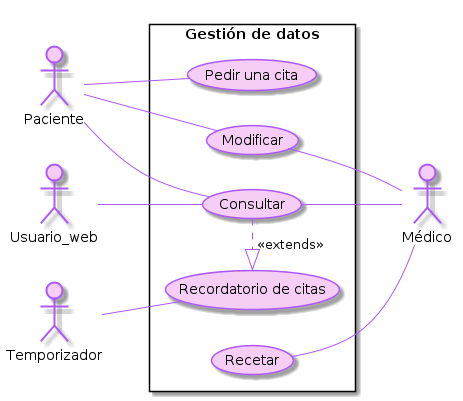
\includegraphics{diagramas/gestion_datos}
\end{figure}

\begin{figure}[H]
	\caption{Diagrama de casos de uso de contabilidad}
	\centering
	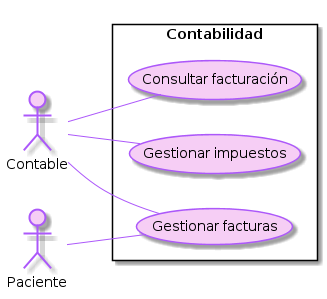
\includegraphics{diagramas/contabilidad}
\end{figure}

\section{Descripción de los actores}
% PLANTILLA PACIENTE

\begin{table}[H]
\label{my-label}
\begin{tabularx}{\textwidth}{l|Xlllr}
	\textbf{Actor}           & \multicolumn{4}{l}{Paciente} & \act\\ 
	\textbf{Descripción}     & \multicolumn{5}{>{\hsize=\dimexpr\textwidth-\hsize\relax}X}{Paciente adscrito al centro médico que desea pedir cita, consultar su historial, informarse acerca de la clínica y gestionar sus facturas}\\
	\textbf{Características} & \multicolumn{5}{>{\hsize=2\hsize}X}{Todos los clientes de la clínica son pacientes}\\ 
	\textbf{Relaciones}      & \multicolumn{5}{>{\hsize=2\hsize}X}{No tiene}\\ 
	\textbf{Referencias}     & \multicolumn{5}{>{\hsize=2\hsize}X}{Pedir una cita, modificar, consultar, gestionar facturas}\\
	\textbf{Autor}           & Grupo ? & \textbf{Fecha} & 07/04/18 & \textbf{Versión} & {1.1}                      \\ 
\end{tabularx}
\end{table}

\begin{table}[H]
\label{my-label}
\begin{tabularx}{\textwidth}{lXl}
	\textbf{Atributos} &  & \\
	\textbf{Nombre}    & \textbf{Descripción} & \textbf{Tipo} \\ \hline
	Datos personales   & Identifican al paciente (\texttt{Id\_paciente}, DNI, nombre y apellidos, ...)     & \\
	Contacto           & Permiten ponerse en contacto con el paciente o algún familiar (teléfono, en caso de emergencia avisar a ...) & \\  
	Datos médicos      & Información relativa a la salud del paciente (historial médico, grupo sanguíneo, enfermedades previas, alergias, ...)            
\end{tabularx}
\end{table}

\begin{table}[H]
\begin{tabularx}{\textwidth}{X}
	\textbf{Comentarios}\\ \hline
\end{tabularx}
\end{table}
% FIN PLANTILLA PACIENTE

\newpage

% PLANTILLA MÉDICO

\begin{table}[H]
\label{my-label}
\begin{tabularx}{\textwidth}{l|Xlllr}
	\textbf{Actor}           & Médico & & & & \act \\ 
	\textbf{Descripción}     & \multicolumn{5}{>{\hsize=\dimexpr\textwidth-\hsize\relax}X}{Personal sanitario de la clínica que se encarga de atender a los pacientes en las consultas}\\
	\textbf{Características} & \multicolumn{5}{>{\hsize=\dimexpr\textwidth-\hsize\relax}X}{Puede consultar y modificar la información del paciente además de recetar medicamentos a los pacientes}\\ 
	\textbf{Relaciones}      & \multicolumn{5}{>{\hsize=\dimexpr\textwidth-\hsize\relax}X}{No tiene}\\ 
	\textbf{Referencias}     & \multicolumn{5}{>{\hsize=\dimexpr\textwidth-\hsize\relax}X}{Modificar, Recetar}\\ 
	\textbf{Autor}           & Grupo ? & \textbf{Fecha} & 07/04/18 & \textbf{Versión} & 1.0\\ 
\end{tabularx}
\end{table}

\begin{table}[H]
\label{my-label}
\begin{tabularx}{\textwidth}{lXl}
	\textbf{Atributos} &  & \\
	\textbf{Nombre}    & \textbf{Descripción} & \textbf{Tipo} \\ \hline
	Datos personales   &  Identifican al médico (\texttt{Id\_médico}, DNI, nombre y apellidos, ...)     & \\
	Datos laborales    & Relativos a su trabajo (horario, sueldo, vacaciones,...) &
\end{tabularx}
\end{table}

\begin{table}[H]
\begin{tabularx}{\textwidth}{X}
	\textbf{Comentarios}\\ \hline
	Los médicos son los únicos que pueden recetar
\end{tabularx}
\end{table}

% FIN PLANTILLA MÉDICO

\newpage

% PLANTILLA CONTABLE

\begin{table}[H]
	\label{my-label}
	\begin{tabularx}{\textwidth}{l|Xlllr}
		\textbf{Actor}           & \multicolumn{4}{l}{Contable} & \act\\ 
		\textbf{Descripción}     & \multicolumn{5}{>{\hsize=\dimexpr\textwidth-\hsize\relax}X}{Encargado de gestionar la facturación y los impuestos referentes a la clínica}\\
		\textbf{Características} & \multicolumn{5}{>{\hsize=\dimexpr\textwidth-\hsize\relax}X}{Puede consultar las facturas de todo cliente en el sistema y el sueldo del personal, así como etiquetar como moroso a aquel cliente que debe dinero}\\ 
		\textbf{Relaciones}      & \multicolumn{5}{>{\hsize=\dimexpr\textwidth-\hsize\relax}X}{No tiene}\\ 
		\textbf{Referencias}     & \multicolumn{5}{>{\hsize=\dimexpr\textwidth-\hsize\relax}X}{Consultar facturación, gestionar impuestos, gestionar facturas}\\
		\textbf{Autor}           & Grupo ? & \textbf{Fecha} & 04/04/18 & \textbf{Versión} & 1.1                    \\ 
	\end{tabularx}
\end{table}

\begin{table}[H]
	\label{my-label}
	\begin{tabularx}{\textwidth}{lXl}
		\textbf{Atributos}  &  & \\
		\textbf{Nombre}     & \textbf{Descripción} & \textbf{Tipo} \\ \hline
		IdContable & Nombre o pseudónimo referente al contable, único en el sistema que identificará a este & Texto \\
		Salario    & Cantidad de dinero que cobra el contable al mes & Numérico \\
	\end{tabularx}
\end{table}

\begin{table}[H]
	\begin{tabularx}{\textwidth}{X}
		\textbf{Comentarios}\\ \hline
		Usualmente no habrá más de un contable por clínica
	\end{tabularx}
\end{table}

%FIN DE LA PLANTILLA CONTABLE

\newpage

% PLANTILLA USUARIO WEB

\begin{table}[H]
	\label{my-label}
	\begin{tabularx}{\textwidth}{l|Xlllr}
		\textbf{Actor}           & \multicolumn{4}{l}{Usuario web} & \act\\ 
		\textbf{Descripción}     & \multicolumn{5}{>{\hsize=\dimexpr\textwidth-\hsize\relax}X}{Cualquier persona que acceda a la información disponible en la página web}\\
		\textbf{Características} & \multicolumn{5}{>{\hsize=\dimexpr\textwidth-\hsize\relax}X}{Puede acceder a diversa información tal como las especialidades, tratamientos, horarios, instalaciones o médicos disponibles}\\ 
		\textbf{Relaciones}      & \multicolumn{5}{>{\hsize=\dimexpr\textwidth-\hsize\relax}X}{No tiene}\\ 
		\textbf{Referencias}     & \multicolumn{5}{>{\hsize=\dimexpr\textwidth-\hsize\relax}X}{Consultar}\\
		\textbf{Autor}           & Grupo ? & \textbf{Fecha} & 04/04/18 & \textbf{Versión} & 1.1.1                      \\ 
	\end{tabularx}
\end{table}

\begin{table}[H]
	\begin{tabularx}{\textwidth}{X}
		\textbf{Comentarios}\\\hline
		No se va a guardar información sobre estos usuarios, puede ser cualquier persona que quiera informarse sobre la clínica
	\end{tabularx}
\end{table}

% FIN DE LA PLANTILLA USUARIO WEB

\newpage

% PLANTILLA TEMPORIZADOR

\begin{table}[H]
	\label{my-label}
	\begin{tabularx}{\textwidth}{l|Xlllr}
		\textbf{Actor}           & \multicolumn{4}{l}{Temporizador} & \act\\ 
		\textbf{Descripción}     & \multicolumn{5}{>{\hsize=\dimexpr\textwidth-\hsize\relax}X}{\textit{Daemon} cuyo objetivo es recordar las citas a los demás usuarios del sistema}\\
		\textbf{Características} & \multicolumn{5}{>{\hsize=\dimexpr\textwidth-\hsize\relax}X}{Accede a los horarios de los distintos usuarios del sistema de forma periódica y avisa tanto a clientes como a trabajadores de su horario}\\ 
		\textbf{Relaciones}      & \multicolumn{5}{>{\hsize=\dimexpr\textwidth-\hsize\relax}X}{No tiene}\\ 
		\textbf{Referencias}     & \multicolumn{5}{>{\hsize=\dimexpr\textwidth-\hsize\relax}X}{Recordatorio de citas}\\
		\textbf{Autor}           & Grupo ? & \textbf{Fecha} & 05/04/18 & \textbf{Versión} & 1.1                     \\ 
	\end{tabularx}
\end{table}

\begin{table}[H]
	\begin{tabularx}{\textwidth}{X}
		\textbf{Comentarios}\\ \hline
		Sobre este actor tampoco se almacena información debido a sus funcionalidades
	\end{tabularx}
\end{table}

% FIN DE LA PLANTILLA TEMPORIZADOR

\newpage

\section{Descripción de los casos de uso}

% PEDIR CITA

\begin{table}[H]
	\begin{tabularx}{\textwidth}{l|Xlllr}
		\textbf{Caso de Uso}   & Pedir cita & & & & \cu \\  
		\textbf{Actores}       & Paciente & & & \\ 
		\textbf{Tipo}          & Primario & & & \\
		\textbf{Referencias}   & RF-1, RN-1, RN-2, RI-1 & & & \\
		\textbf{Precondición}  & \multicolumn{5}{>{\hsize=\dimexpr\textwidth-0.85\hsize\relax}X}{Plataforma activa y operativa, paciente correctamente identificado}\\ 
		\textbf{Postcondición} & Cita añadida al sistema & & & & \\
		\textbf{Autor}         & Grupo ? & \textbf{Fecha} & 07/04/18 & \textbf{Versión} & 1.0 \\ 
	\end{tabularx}
\end{table}

\begin{table}[H]
	\begin{tabularx}{\textwidth}{X}
		\textbf{Propósito}\\ \hline
		Permitir que un paciente reserve una cita con su médico
	\end{tabularx}
\end{table}

\begin{table}[H]
	\begin{tabularx}{\textwidth}{X}
		\textbf{Resumen}\\ \hline
		Tras la identificación del paciente éste podrá observar en qué fecha y horario su médico tiene citas disponibles y seleccionar una de ellas, el sistema la marcará como reservada por este paciente
	\end{tabularx}
\end{table}

% FIN PEDIR CITA

\newpage

% CONSULTAR

\begin{table}[H]
	\begin{tabularx}{\textwidth}{l|Xlllr}
		\textbf{Caso de Uso}   & Consultar & & & & \cu \\  
		\textbf{Actores}       & \multicolumn{5}{>{\hsize=\dimexpr\textwidth-\hsize\relax}X}{Paciente, médico, usuario web, administrador}\\ 
		\textbf{Tipo}          & Primario, esencial & & & \\
		\textbf{Referencias}   & \multicolumn{5}{>{\hsize=\dimexpr\textwidth-\hsize\relax}X}{RF-2, RF-4, RF-5, RF-7, RF-8, RF-13, RF-14, RF-15, RF-27, RF-30, RN-1, RN-4, RN-6}\\
		\textbf{Precondición}  & \multicolumn{5}{>{\hsize=\dimexpr\textwidth-0.85\hsize\relax}X}{Plataforma activa y operativa, usuario y/o médico registrados en el sistema}\\ 
		\textbf{Postcondición} & - & & & & \\
		\textbf{Autor}         & Grupo ? & \textbf{Fecha} & 07/04/18 & \textbf{Versión} & 1.0 \\ 
	\end{tabularx}
\end{table}

\begin{table}[H]
	\begin{tabularx}{\textwidth}{X}
		\textbf{Propósito}\\ \hline
		Permitir tanto a pacientes como a médicos acceder al historial clínico de los pacientes, entre otros datos como los medicamentos recetados o las listas de espera

		Permite al usuario web acceder a diversa información tal como las especialidades, tratamientos, horarios, instalaciones o médicos disponibles

		También permite al administrador consultar todas las bases de datos del sistema
	\end{tabularx}
\end{table}

\begin{table}[H]
	\begin{tabularx}{\textwidth}{X}
		\textbf{Resumen}\\ \hline
		El usuario accede a la aplicación, se identifica y solicita acceder a su ficha médica, si es paciente, o a la de un paciente cualquiera, si es médico. En esta ficha se puede consultar el historial clínico, los medicamentos recetados o las listas de espera, entre otros datos.

		El usuario web accede a la web y sin necesidad de identificarse puede consultar la información sobre la clínica disponible públicamente

		El administrador cuenta con una interfaz específica desde la que puede consultar todas las bases de datos del sistema 
	\end{tabularx}
\end{table}

% FIN DE CONSULTAR

\newpage

% MODIFICAR

\begin{table}[H]
	\begin{tabularx}{\textwidth}{l|Xlllr}
		\textbf{Caso de Uso}   & Modificar & & & & \cu \\  
		\textbf{Actores}       & Paciente, médico & & & \\ 
		\textbf{Tipo}          & Primario, esencial & & & \\
		\textbf{Referencias}   & \multicolumn{5}{>{\hsize=\dimexpr\textwidth-\hsize\relax}X}{RF-2, RF-9, RF-13, RF-15, RNF-1, RNF-2}\\
		\textbf{Precondición}  & \multicolumn{5}{>{\hsize=\dimexpr\textwidth-0.85\hsize\relax}X}{Plataforma activa y operativa, usuario y/o médico registrados en el sistema.}\\ 
		\textbf{Postcondición} & - & & & & \\
		\textbf{Autor}         & Grupo ? & \textbf{Fecha} & 05/04/18 & \textbf{Versión} & 1.1 \\ 
	\end{tabularx}
\end{table}

\begin{table}[H]
	\begin{tabularx}{\textwidth}{X}
		\textbf{Propósito}\\ \hline
		Dar la posibilidad de modificar los datos sobre un elemento del sistema tras haberlos introducido en su registro si se tiene permiso para ello
	\end{tabularx}
\end{table}

\begin{table}[H]
	\begin{tabularx}{\textwidth}{X}
		\textbf{Resumen}\\ \hline
		El usuario accede a su ficha médica (o el médico a la de éste) y solicita editar sus datos. En caso de que se acepte la petición, puede introducir los nuevos y aceptar la modificación de éstos. También pueden modificarse las listas de espera y el horario de los médicos de igual manera
	\end{tabularx}
\end{table}

% FIN DE MODIFICAR

\newpage

% INICIO DE RECETAR

\begin{table}[H]
	\begin{tabularx}{\textwidth}{l|Xlllr}
		\textbf{Caso de Uso}   & Recetar & & & & \cu \\  
		\textbf{Actores}       & Médico & & & \\ 
		\textbf{Tipo}          & Primario, esencial & & & \\
		\textbf{Referencias}   & \multicolumn{5}{>{\hsize=\dimexpr\textwidth-\hsize\relax}X}{RF-12}\\
		\textbf{Precondición}  & \multicolumn{5}{>{\hsize=\dimexpr\textwidth-0.85\hsize\relax}X}{Plataforma activa y operativa, médico registrado en el sistema}\\ 
		\textbf{Postcondición} & \multicolumn{5}{>{\hsize=\dimexpr\textwidth-0.85\hsize\relax}X}{Historial médico correctamente modificado}\\
		\textbf{Autor}         & Grupo ? & \textbf{Fecha} & 05/04/18 & \textbf{Versión} & 1.0 \\ 
	\end{tabularx}
\end{table}

\begin{table}[H]
	\begin{tabularx}{\textwidth}{X}
		\textbf{Propósito}\\ \hline
		El médico receta al paciente las medicinas que necesite (añadidas al historial médico)
	\end{tabularx}
\end{table}

\begin{table}[H]
	\begin{tabularx}{\textwidth}{X}
		\textbf{Resumen}\\ \hline
		Seleccionado el paciente al que se le va a recetar, el médico solicita ver la lista de recetas disponibles poniendo un filtro adecuado si lo cree necesario (como por nombre, tipo...). El sistema le devuelve la lista de medicamentos disponibles, y el médico selecciona las recetas oportunas, cargándose éstas al historial médico del paciente
	\end{tabularx}
\end{table}

% FIN RECETAR

\newpage

% INICIO DE GESTIÓN DE IMPUESTOS

\begin{table}[H]
	\begin{tabularx}{\textwidth}{l|Xlllr}
		\textbf{Caso de Uso}   & Gestionar impuestos & & & & \cu \\  
		\textbf{Actores}       & Contable & & & \\ 
		\textbf{Tipo}          & Primario, esencial & & & \\
		\textbf{Referencias}   & \multicolumn{5}{>{\hsize=\dimexpr\textwidth-\hsize\relax}X}{RF-25, RNF-1, Consultar}\\
		\textbf{Precondición}  & \multicolumn{5}{>{\hsize=\dimexpr\textwidth-0.85\hsize\relax}X}{Plataforma activa y operativa, acceso al sistema con una usuario contable para gestionar los impuestos}\\ 
		\textbf{Postcondición} & \multicolumn{5}{>{\hsize=\dimexpr\textwidth-0.85\hsize\relax}X}{Notificar al gerente de la modificación de la contabilidad en la clínica}\\
		\textbf{Autor}         & Grupo ? & \textbf{Fecha} & 06/04/18 & \textbf{Versión} & 1.0 \\ 
	\end{tabularx}
\end{table}

\begin{table}[H]
	\begin{tabularx}{\textwidth}{X}
		\textbf{Propósito}\\ \hline
		Facilitar al contable la gestión de los impuestos referentes a la clínica, pudiendo gestionar la contabilidad mediante el sistema informático
	\end{tabularx}
\end{table}

\begin{table}[H]
	\begin{tabularx}{\textwidth}{X}
		\textbf{Resumen}\\ \hline
		El contable entra al sistema mediante su cuenta de contable y accede al apartado de gestión de impuestos, donde podrá dividir el dinero de la clínica en los distintos apartados posibles (investigación, compra de material...). Tras esto, se enviará una notificación al gerente de que se han modificado las cuentas del hospital
	\end{tabularx}
\end{table}

% FIN DE GESTIÓN DE IMPUESTOS

\newpage

% INICIO CONSULTAR FACTURACION

\begin{table}[H]
	\begin{tabularx}{\textwidth}{l|Xlllr}
		\textbf{Caso de Uso}   & Consultar facturación & & & & \cu \\  
		\textbf{Actores}       & Contable & & & \\ 
		\textbf{Tipo}          & Primario, esencial & & & \\
		\textbf{Referencias}   & \multicolumn{5}{>{\hsize=\dimexpr\textwidth-\hsize\relax}X}{RF-5, RF-24, RF-26}\\
		\textbf{Precondición}  & \multicolumn{5}{>{\hsize=\dimexpr\textwidth-0.85\hsize\relax}X}{Plataforma activa y operativa}\\ 
		\textbf{Postcondición} & \multicolumn{5}{>{\hsize=\dimexpr\textwidth-0.85\hsize\relax}X}{-}\\
		\textbf{Autor}         & Grupo ? & \textbf{Fecha} & 06/04/18 & \textbf{Versión} & 1.0 \\ 
	\end{tabularx}
\end{table}

\begin{table}[H]
	\begin{tabularx}{\textwidth}{X}
		\textbf{Propósito}\\ \hline
		Visualizar la facturación de la clínica y las tareas en las que se ha invertido el dinero de ésta
	\end{tabularx}
\end{table}

\begin{table}[H]
	\begin{tabularx}{\textwidth}{X}
		\textbf{Resumen}\\ \hline
		El contable entra al sistema mediante su cuenta de contable y accede al apartado consultar facturación, donde aparecerán distintas tablas con la facturación referente a la clínica
	\end{tabularx}
\end{table}

% FIN CONSULTAR FACTURACIÓN

\newpage

% INICIO DE GESTIONAR FACTURAS

\begin{table}[H]
	\begin{tabularx}{\textwidth}{l|Xlllr}
		\textbf{Caso de Uso}   & Gestionar facturas & & & & \cu \\  
		\textbf{Actores}       & Contable, paciente & & & \\ 
		\textbf{Tipo}          & Primario, esencial & & & \\
		\textbf{Referencias}   & \multicolumn{5}{>{\hsize=\dimexpr\textwidth-\hsize\relax}X}{RF-5, RF-24, RF-26, RNF-1}\\
		\textbf{Precondición}  & \multicolumn{5}{>{\hsize=\dimexpr\textwidth-0.85\hsize\relax}X}{Plataforma activa y operativa, factura a la que se quiere acceder registrada en el sistema}\\ 
		\textbf{Postcondición} & \multicolumn{5}{>{\hsize=\dimexpr\textwidth-0.85\hsize\relax}X}{Facturas correctamente modificadas. En caso de que el contable etiquete como moroso a un paciente por no haber pagado, notificar al paciente}\\
		\textbf{Autor}         & Grupo ? & \textbf{Fecha} & 06/04/18 & \textbf{Versión} & 1.0 \\ 
	\end{tabularx}
\end{table}

\begin{table}[H]
	\begin{tabularx}{\textwidth}{X}
		\textbf{Propósito}\\ \hline
		Dar la opción al paciente para que gestione su seguro médico referente a la clínica mediante el sistema informático, haciendo que no se tenga que desplazar a la clínica para gestionar sus facturas

		Por parte del contable, gestionar las distintas facturas de cada paciente para comprobar que todas están pagadas y bien establecidas
	\end{tabularx}
\end{table}

\begin{table}[H]
	\begin{tabularx}{\textwidth}{X}
		\textbf{Resumen}\\ \hline
		El paciente o el contable acceden al sistema mediante su usuario y seleccionan el apartado gestionar facturas, donde aparecerán sus facturas ordenadas junto a distintas opciones a realizar sobre ellas. 

		El contable podrá hacer una búsqueda sobre todas las facturas del sistema y gestionar la de cualquier paciente
	\end{tabularx}
\end{table}

% FIN DE GESTIONAR FACTURAS

\newpage

% INICIO DE RECORDATORIO DE CITAS

\begin{table}[H]
	\begin{tabularx}{\textwidth}{l|Xlllr}
		\textbf{Caso de Uso}   & Recordatorio de citas & & & & \cu \\  
		\textbf{Actores}       & Temporizador & & & \\ 
		\textbf{Tipo}          & Opcional & & & \\
		\textbf{Referencias}   & \multicolumn{5}{>{\hsize=\dimexpr\textwidth-\hsize\relax}X}{RF-6, RN-3}\\
		\textbf{Precondición}  & \multicolumn{5}{>{\hsize=\dimexpr\textwidth-0.85\hsize\relax}X}{Plataforma activa y operativa, servicio de mensajería activo y existencia de cita a recordar}\\ 
		\textbf{Postcondición} & \multicolumn{5}{>{\hsize=\dimexpr\textwidth-0.85\hsize\relax}X}{Recordatorio correctamente enviado.}\\
		\textbf{Autor}         & Grupo ? & \textbf{Fecha} & 07/04/18 & \textbf{Versión} & 1.0 \\ 
	\end{tabularx}
\end{table}

\begin{table}[H]
	\begin{tabularx}{\textwidth}{X}
		\textbf{Propósito}\\ \hline
		Recordar al paciente que tiene una cita. Este acción se puede regular dependiendo del paciente si este quiere que se le notifique o no, con qué regularidad o con cuánta antelación
	\end{tabularx}
\end{table}

\begin{table}[H]
	\begin{tabularx}{\textwidth}{X}
		\textbf{Resumen}\\ \hline
		Se inicia el proceso del temporizador (ya sea de forma periódica o a una hora programada), consulta las citas programadas y envía un recordatorio a aquellos clientes que así lo tengan especificado, cumpliendo restricciones de tiempo especificadas por los mismos
	\end{tabularx}
\end{table}

% FIN DE RECORDATORIO DE CITAS

\newpage


% FIN DE RECETAR

\newpage
\section{Diagrama de paquetes}

\begin{figure}[H]
	\caption{Diagrama de paquetes}
	\centering
	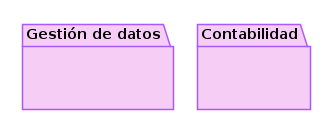
\includegraphics{diagramas/paquetes}
\end{figure}
	
	
\end{document}
